% Options for packages loaded elsewhere
\PassOptionsToPackage{unicode}{hyperref}
\PassOptionsToPackage{hyphens}{url}
%
\documentclass[
  12pt,a4paper,lualatex,ja=standard]{bxjsarticle}
\usepackage{lmodern}
\usepackage{amsmath}
\usepackage{ifxetex,ifluatex}
\ifnum 0\ifxetex 1\fi\ifluatex 1\fi=0 % if pdftex
  \usepackage[T1]{fontenc}
  \usepackage[utf8]{inputenc}
  \usepackage{textcomp} % provide euro and other symbols
  \usepackage{amssymb}
\else % if luatex or xetex
  \usepackage{unicode-math}
  \defaultfontfeatures{Scale=MatchLowercase}
  \defaultfontfeatures[\rmfamily]{Ligatures=TeX,Scale=1}
\fi
% Use upquote if available, for straight quotes in verbatim environments
\IfFileExists{upquote.sty}{\usepackage{upquote}}{}
\IfFileExists{microtype.sty}{% use microtype if available
  \usepackage[]{microtype}
  \UseMicrotypeSet[protrusion]{basicmath} % disable protrusion for tt fonts
}{}
\makeatletter
\@ifundefined{KOMAClassName}{% if non-KOMA class
  \IfFileExists{parskip.sty}{%
    \usepackage{parskip}
  }{% else
    \setlength{\parindent}{0pt}
    \setlength{\parskip}{6pt plus 2pt minus 1pt}}
}{% if KOMA class
  \KOMAoptions{parskip=half}}
\makeatother
\usepackage{xcolor}
\IfFileExists{xurl.sty}{\usepackage{xurl}}{} % add URL line breaks if available
\IfFileExists{bookmark.sty}{\usepackage{bookmark}}{\usepackage{hyperref}}
\hypersetup{
  hidelinks,
  pdfcreator={LaTeX via pandoc}}
\urlstyle{same} % disable monospaced font for URLs
\usepackage{graphicx}
\makeatletter
\def\maxwidth{\ifdim\Gin@nat@width>\linewidth\linewidth\else\Gin@nat@width\fi}
\def\maxheight{\ifdim\Gin@nat@height>\textheight\textheight\else\Gin@nat@height\fi}
\makeatother
% Scale images if necessary, so that they will not overflow the page
% margins by default, and it is still possible to overwrite the defaults
% using explicit options in \includegraphics[width, height, ...]{}
\setkeys{Gin}{width=\maxwidth,height=\maxheight,keepaspectratio}
% Set default figure placement to htbp
\makeatletter
\def\fps@figure{htbp}
\makeatother
\setlength{\emergencystretch}{3em} % prevent overfull lines
\providecommand{\tightlist}{%
  \setlength{\itemsep}{0pt}\setlength{\parskip}{0pt}}
\setcounter{secnumdepth}{5}
\usepackage{indentfirst}
\parindent = 1em
\usepackage{dcolumn}
\newcolumntype{.}{D{.}{.}{-1}}
\usepackage{caption}
\captionsetup[table]{name=表}
\captionsetup[figure]{name=図}
\usepackage{hyperref}
\pagestyle{empty}
\usepackage{multicol}
\usepackage{ascmac}
\setpagelayout*{top=10truemm,bottom=30truemm,left=10truemm,right=10truemm}
\usepackage{tikz}
\usetikzlibrary{arrows.meta,decorations,decorations.pathreplacing,arrows,calc}
\usepackage{tabstackengine}
\usepackage{xcolor}
\usepackage{rotating}
\usepackage{txfonts}
\usepackage{fancybox}
\usepackage{dashbox}
\usepackage{tcolorbox}
\tcbuselibrary{theorems,skins}
\usepackage{siunitx}
\usepackage{framed}
\usepackage{enumerate}
\usepackage{lastpage}
\usepackage{pgfplots}
\pgfplotsset{compat=1.15}
\usepackage{mathrsfs}
\ifluatex
  \usepackage{selnolig}  % disable illegal ligatures
\fi

\author{}
\date{\vspace{-2.5em}}

\begin{document}

\renewcommand{\thefootnote}{}
\newcounter{kaunta}
\renewcommand{\thekaunta}{\arabic{kaunta}}
\newcommand{\kaunta}{\refstepcounter{kaunta}%
\thekaunta}
\def\question{\noindent\fbox{\large\makebox[1em]{\text{\kaunta}}} \hspace{1pt}}
\newcounter{skaunta}
\renewcommand{\theskaunta}{\arabic{skaunta}}
\newcommand{\skaunta}{\refstepcounter{skaunta}%
\theskaunta}
\def\squestion{(\text{\skaunta})\hspace{2.5pt}}
\newcommand{\maru}[1]{\raise0.2ex\hbox{\textcircled{\scriptsize{#1}}}}
\newcommand{\jsim}{\mathrel{\text{∽}}}
\newcommand{\jpara}{/\!/}

\newcounter{kcounter}
\setcounter{kcounter}{0}
\newcommand{\kana}{\refstepcounter{kcounter}\ifthenelse{\value{kcounter}=1}{ア}{\ifthenelse{\value{kcounter}=2}{イ}{\ifthenelse{\value{kcounter}=3}{ウ}{\ifthenelse{\value{kcounter}=4}{エ}{\ifthenelse{\value{kcounter}=5}{オ} {\ifthenelse{\value{kcounter}=6}{カ}{\ifthenelse{\value{kcounter}=7}{キ}{\ifthenelse{\value{kcounter}=8}{ク}{\ifthenelse{\value{kcounter}=9}{ケ}{\ifthenelse{\value{kcounter}=10}{コ}{\ifthenelse{\value{kcounter}=11}{サ}{\ifthenelse{\value{kcounter}=12}{シ}{\ifthenelse{\value{kcounter}=13}{ス}{\ifthenelse{\value{kcounter}=14}{セ}{\ifthenelse{\value{kcounter}=15}{ソ}{\ifthenelse{\value{kcounter}=16}{タ}{\ifthenelse{\value{kcounter}=17}{チ}{\ifthenelse{\value{kcounter}=18}{ツ}{\ifthenelse{\value{kcounter}=19}{テ}{\ifthenelse{\value{kcounter}=20}{ト}{\ifthenelse{\value{kcounter}=21}{ナ}{\ifthenelse{\value{kcounter}=22}{ニ}{\ifthenelse{\value{kcounter}=23}{ヌ}{\ifthenelse{\value{kcounter}=24}{ネ}{\ifthenelse{\value{kcounter}=25}{ノ}{\ifthenelse{\value{kcounter}=26}{ハ}{\ifthenelse{\value{kcounter}=27}{ヒ}{\ifthenelse{\value{kcounter}=28}{フ}{\ifthenelse{\value{kcounter}=29}{ヘ}{\ifthenelse{\value{kcounter}=30}{ホ}{\ifthenelse{\value{kcounter}=31}{マ}{\ifthenelse{\value{kcounter}=32}{ミ}{\ifthenelse{\value{kcounter}=33}{ム}{\ifthenelse{\value{kcounter}=34}{メ}{\ifthenelse{\value{kcounter}=35}{モ}{\ifthenelse{\value{kcounter}=36}{ヤ}{\ifthenelse{\value{kcounter}=37}{ユ}{\ifthenelse{\value{kcounter}=38}{ヨ}{\ifthenelse{\value{kcounter}=39}{ラ}{\ifthenelse{\value{kcounter}=40}{リ}{\ifthenelse{\value{kcounter}=41}{ル}{\ifthenelse{\value{kcounter}=42}{レ}{\ifthenelse{\value{kcounter}=43}{ロ}{\ifthenelse{\value{kcounter}=44}{ワ}{・}}}}}}}}}}}}}}}}}}}}}}}}}}}}}}}}}}}}}}}}}}}}}

\newcommand{\kuran}[1]{\framebox[1.5cm][c]{\maru{\kana}}}

\newcommand{\degre}{\ensuremath{^\circ}}

\newcommand{\myarc}[1]{
   \tikz [baseline = (N.base), every node/.style={}] {
      \node [inner sep = 0pt] (N) {$\mathrm{#1}$};
      \draw [line width = 0.4pt] plot [smooth, tension=1.3] coordinates {
         ($(N.north west) + (0.1ex,0)$)
         ($(N.north)      + (0,0.5ex)$)
         ($(N.north east) + (0,0)$)
      };
   }
}

\makeatletter
\newenvironment{figurehere}{\def\@captype{figure}}{}
\makeatother

\newcommand{\haiten}[1]{%
\begin{flushright}%
\footnotesize{<#1>}%
\end{flushright}%
}
\newgeometry{top=10truemm,bottom=10truemm,left=20truemm,right=20truemm}

\thispagestyle{empty}
\begin{center}
\phantom{empty}

\vspace{60truemm}

\hspace{4em} {\HUGE\gtfamily\bfseries 数\hspace{2em}学}\hspace{1em}{\large \gtfamily \bfseries ($\mathbf{2}$年)}\\

\vspace{15truemm}

\hspace{2.5em}{\large \gtfamily \bfseries (この問題は定規とコンパスが必要です。)}

\vspace{64truemm}

{\large\gtfamily\bfseries 注\hspace{5em}意}

\end{center}

\centering
\begin{framed}
\begin{flushleft}
\begin{enumerate}[\Large \gtfamily 1]
  \item {\large 「開始」の合図があるまでは,開いてはいけません。}

  \item {\large 問題は\pageref{LastPage}ページまであります。}

  \item {\large 「開始」の合図があったら,まず,問題用紙・解答用紙に,組・番号と名前などを書きなさい。}

  \item {\large 答えは,すべて解答用紙に書きなさい。また、所定の欄に濃くはっきりと書きなさい。}

  \item {\large 「終了」の合図で,すぐ鉛筆をおき,解答用紙を裏返しにしなさい。}
\end{enumerate}
\end{flushleft}
\end{framed}

\vspace{14mm}

\begin{center}
{\large \underline{\hspace{30mm}組 \hspace{30mm}番 \hspace{15mm} 名前 \hspace{60mm}}}
\end{center}

\newpage

  \href{空白ページのための全角スペースあり。}{} \newpage

\pagestyle{plain}
\pagenumbering{arabic}

\begin{flushleft}

\noindent\fbox{\large\makebox[1em]{\text{\refstepcounter{kaunta}%
\arabic{kaunta}}}} \hspace{1pt}次の各問に答えなさい。

%
\begin{flushright}%
\footnotesize{<知・技$2 \times 4$点>}%
\end{flushright}%


(\text{\refstepcounter{skaunta}%
\arabic{skaunta}})\hspace{2.5pt}二等辺三角形の定義をかけ。

(\text{\refstepcounter{skaunta}%
\arabic{skaunta}})\hspace{2.5pt}正三角形の定義をかけ。

(\text{\refstepcounter{skaunta}%
\arabic{skaunta}})\hspace{2.5pt}直角三角形の合同条件を2つかけ。

\vfill

\setcounter{skaunta}{0}

\noindent\fbox{\large\makebox[1em]{\text{\refstepcounter{kaunta}%
\arabic{kaunta}}}} \hspace{1pt}次の$\angle x$の大きさを求めなさい。

%
\begin{flushright}%
\footnotesize{<知・技$3 \times 8$点>}%
\end{flushright}%


\begin{multicols}{2}
(\text{\refstepcounter{skaunta}%
\arabic{skaunta}})\hspace{2.5pt}

\begin{center}
\def\@captype{figure}
\includegraphics[height=22mm]{media/tu1.jpg}

\end{center}

\columnbreak

(\text{\refstepcounter{skaunta}%
\arabic{skaunta}})\hspace{2.5pt}

\begin{center}
\def\@captype{figure}
\includegraphics[height=22mm]{media/tu2.jpg}

\end{center}

\end{multicols}

\vspace{5mm}

\begin{multicols}{2}
(\text{\refstepcounter{skaunta}%
\arabic{skaunta}})\hspace{2.5pt}

\begin{center}
\def\@captype{figure}
\includegraphics[height=35mm]{media/tu3.jpg}

\end{center}

\columnbreak

(\text{\refstepcounter{skaunta}%
\arabic{skaunta}})\hspace{2.5pt}

\begin{center}
\def\@captype{figure}
\includegraphics[height=35mm]{media/tu6.jpg}

\end{center}

\end{multicols}

\vspace{5mm}


\begin{multicols}{2}
(\text{\refstepcounter{skaunta}%
\arabic{skaunta}})\hspace{2.5pt}

\begin{center}
\def\@captype{figure}
\includegraphics[height=22mm]{media/tu7.jpg}

\end{center}

\columnbreak

(\text{\refstepcounter{skaunta}%
\arabic{skaunta}})\hspace{2.5pt}

\begin{center}
\def\@captype{figure}
\includegraphics[height=28mm]{media/tu8.jpg}

\end{center}

\end{multicols}

\vspace{5mm}

\begin{multicols}{2}
(\text{\refstepcounter{skaunta}%
\arabic{skaunta}})\hspace{2.5pt}$l /\!/m$

\begin{center}
\def\@captype{figure}
\includegraphics[height=30mm]{media/tu9.jpg}

\end{center}

\columnbreak

(\text{\refstepcounter{skaunta}%
\arabic{skaunta}})\hspace{2.5pt}$\triangle$ABCは正三角形で$l /\!/m$

\begin{center}
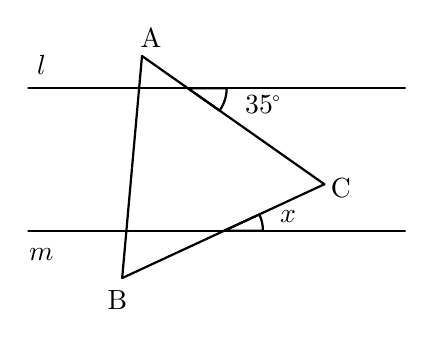
\begin{tikzpicture}[scale=0.6,line cap=round,line join=round,>=triangle 45,x=1.0cm,y=1.0cm]
\clip(-2.,-2.) rectangle (6.,4.3);
\draw [shift={(1.38730940174405,3.02)},line width=0.8pt] (0,0) -- (-35.10648457232839:0.8253747651743738) arc (-35.10648457232839:0.:0.8253747651743738) -- cycle;
\draw [shift={(2.1549541808120143,0.)},line width=0.8pt] (0,0) -- (0.:0.8253747651743738) arc (0.:24.893515427671613:0.8253747651743738) -- cycle;
\draw [line width=0.8pt,domain=-2.:6.] plot(\x,{(-0.-0.*\x)/5.56});
\draw [line width=0.8pt,domain=-2.:6.] plot(\x,{(--16.7912-0.*\x)/5.56});
\draw [line width=0.8pt] (0.42,3.7)-- (0.,-1.);
\draw [line width=0.8pt] (0.,-1.)-- (4.280319397786862,0.9862693304105346);
\draw [line width=0.8pt] (4.280319397786862,0.9862693304105346)-- (0.42,3.7);
\draw (0.6117616632565556,4.1) node {A};
\draw (-0.1,-1.4576641538312174) node {B};
\draw (4.6285855204385085,0.9084101730019845) node {C};
\draw[color=black] (3.0,2.6692096720406466) node {$35\textrm{\ensuremath{^\circ}}$};
\draw[color=black] (3.5280858335393432,0.30313534520744445) node {$x$};
\draw (-1.7, 3.5) node{$l$};
\draw (-1.7, -0.5) node{$m$};
\end{tikzpicture}
\end{center}
\end{multicols}


\vfill

\newpage

\noindent\fbox{\large\makebox[1em]{\text{\refstepcounter{kaunta}%
\arabic{kaunta}}}} \hspace{1pt}次のそれぞれのことがらについて、逆を答え、正しいか正しくないかに丸をつけなさい。また、正しくないときは反例をあげなさい。

%
\begin{flushright}%
\footnotesize{<知・技$3 \times 5$点>}%
\end{flushright}%


\setcounter{skaunta}{0}

\begin{multicols}{2}
(\text{\refstepcounter{skaunta}%
\arabic{skaunta}})\hspace{2.5pt}右の図で、$\angle a = \angle b$ならば$l /\!/m$

\columnbreak

\begin{center}
\def\@captype{figure}
\includegraphics[height=30mm]{media/tu10.jpg}

\end{center}

\end{multicols}

(\text{\refstepcounter{skaunta}%
\arabic{skaunta}})\hspace{2.5pt}$x \geqq 8$ならば$x > 5$

(\text{\refstepcounter{skaunta}%
\arabic{skaunta}})\hspace{2.5pt}$\triangle$ABCが正三角形ならば$\angle \mbox{A} = \ang{60}$

(\text{\refstepcounter{skaunta}%
\arabic{skaunta}})\hspace{2.5pt}$\triangle$ABCで$\angle \mbox{A} = \ang{90}$ならば$\angle \mbox{B} + \angle \mbox{C} = \ang{90}$

(\text{\refstepcounter{skaunta}%
\arabic{skaunta}})\hspace{2.5pt}整数$a ,\, b$で、$a$も$b$も偶数ならば$ab$は偶数である。

\vfill

\noindent\fbox{\large\makebox[1em]{\text{\refstepcounter{kaunta}%
\arabic{kaunta}}}} \hspace{1pt}下の図で、合同な三角形はどれとどれか。記号$\equiv$を使って表しなさい。また、そのときに使った合同条件を答えなさい。

%
\begin{flushright}%
\footnotesize{<知・技$4 \times 2$点>}%
\end{flushright}%


\begin{center}
\def\@captype{figure}
\includegraphics[height=50mm]{media/image160.png}

\end{center}

\vfill

\noindent\fbox{\large\makebox[1em]{\text{\refstepcounter{kaunta}%
\arabic{kaunta}}}} \hspace{1pt}2つの内角の大きさが次のような三角形の中から、二等辺三角形をすべて選びなさい。

%
\begin{flushright}%
\footnotesize{<知・技4点>}%
\end{flushright}%


$\raise 0.2ex\hbox{\textcircled{\scriptsize{ア}}}$ $\ang{40}, \ang{100}$ \hspace{10mm} $\raise 0.2ex\hbox{\textcircled{\scriptsize{イ}}}$ $\ang{70}, \ang{50}$ \hspace{10mm} $\raise 0.2ex\hbox{\textcircled{\scriptsize{ウ}}}$ $\ang{120}, \ang{35}$ \hspace{10mm} $\raise 0.2ex\hbox{\textcircled{\scriptsize{エ}}}$ $\ang{30}, \ang{75}$ \hspace{10mm} 

\vfill

\newpage

\begin{multicols}{2}
\noindent\fbox{\large\makebox[1em]{\text{\refstepcounter{kaunta}%
\arabic{kaunta}}}} \hspace{1pt}右の図で、直角三角形ABCの斜辺AB上に$\mbox{AD} = \mbox{AC}$となる点Dをとる。点Dを通るABの垂線と辺BCとの交点をEとすると、$\triangle \mbox{ADE} \equiv \triangle \mbox{ACE}$となることを次のように証明した。\fbox{\phantom{空欄}}にあてはまるものを書きいれて、証明を完成させなさい。

%
\begin{flushright}%
\footnotesize{<知・技$4 \times 5$点>}%
\end{flushright}%


\columnbreak

\begin{center}
\def\@captype{figure}
\includegraphics[height=40mm]{media/tu11.jpg}

\end{center}

\end{multicols}
\begin{itembox}[l]{証明}
$\triangle$ADEと$\triangle$ACEにおいて

仮定から
\begin{flalign*}
\angle\mbox{ADE} &= \angle\mbox{ACE} &\\
&= \framebox[1.5cm][c]{\raise 0.2ex\hbox{\textcircled{\scriptsize{\refstepcounter{kcounter}\ifthenelse{\value{kcounter}=1}{ア}{\ifthenelse{\value{kcounter}=2}{イ}{\ifthenelse{\value{kcounter}=3}{ウ}{\ifthenelse{\value{kcounter}=4}{エ}{\ifthenelse{\value{kcounter}=5}{オ} {\ifthenelse{\value{kcounter}=6}{カ}{\ifthenelse{\value{kcounter}=7}{キ}{\ifthenelse{\value{kcounter}=8}{ク}{\ifthenelse{\value{kcounter}=9}{ケ}{\ifthenelse{\value{kcounter}=10}{コ}{\ifthenelse{\value{kcounter}=11}{サ}{\ifthenelse{\value{kcounter}=12}{シ}{\ifthenelse{\value{kcounter}=13}{ス}{\ifthenelse{\value{kcounter}=14}{セ}{\ifthenelse{\value{kcounter}=15}{ソ}{\ifthenelse{\value{kcounter}=16}{タ}{\ifthenelse{\value{kcounter}=17}{チ}{\ifthenelse{\value{kcounter}=18}{ツ}{\ifthenelse{\value{kcounter}=19}{テ}{\ifthenelse{\value{kcounter}=20}{ト}{\ifthenelse{\value{kcounter}=21}{ナ}{\ifthenelse{\value{kcounter}=22}{ニ}{\ifthenelse{\value{kcounter}=23}{ヌ}{\ifthenelse{\value{kcounter}=24}{ネ}{\ifthenelse{\value{kcounter}=25}{ノ}{\ifthenelse{\value{kcounter}=26}{ハ}{\ifthenelse{\value{kcounter}=27}{ヒ}{\ifthenelse{\value{kcounter}=28}{フ}{\ifthenelse{\value{kcounter}=29}{ヘ}{\ifthenelse{\value{kcounter}=30}{ホ}{\ifthenelse{\value{kcounter}=31}{マ}{\ifthenelse{\value{kcounter}=32}{ミ}{\ifthenelse{\value{kcounter}=33}{ム}{\ifthenelse{\value{kcounter}=34}{メ}{\ifthenelse{\value{kcounter}=35}{モ}{\ifthenelse{\value{kcounter}=36}{ヤ}{\ifthenelse{\value{kcounter}=37}{ユ}{\ifthenelse{\value{kcounter}=38}{ヨ}{\ifthenelse{\value{kcounter}=39}{ラ}{\ifthenelse{\value{kcounter}=40}{リ}{\ifthenelse{\value{kcounter}=41}{ル}{\ifthenelse{\value{kcounter}=42}{レ}{\ifthenelse{\value{kcounter}=43}{ロ}{\ifthenelse{\value{kcounter}=44}{ワ}{・}}}}}}}}}}}}}}}}}}}}}}}}}}}}}}}}}}}}}}}}}}}}}}}} \quad \cdots \cdots \raise 0.2ex\hbox{\textcircled{\scriptsize{1}}} &
\end{flalign*}
\framebox[1.5cm][c]{\raise 0.2ex\hbox{\textcircled{\scriptsize{\refstepcounter{kcounter}\ifthenelse{\value{kcounter}=1}{ア}{\ifthenelse{\value{kcounter}=2}{イ}{\ifthenelse{\value{kcounter}=3}{ウ}{\ifthenelse{\value{kcounter}=4}{エ}{\ifthenelse{\value{kcounter}=5}{オ} {\ifthenelse{\value{kcounter}=6}{カ}{\ifthenelse{\value{kcounter}=7}{キ}{\ifthenelse{\value{kcounter}=8}{ク}{\ifthenelse{\value{kcounter}=9}{ケ}{\ifthenelse{\value{kcounter}=10}{コ}{\ifthenelse{\value{kcounter}=11}{サ}{\ifthenelse{\value{kcounter}=12}{シ}{\ifthenelse{\value{kcounter}=13}{ス}{\ifthenelse{\value{kcounter}=14}{セ}{\ifthenelse{\value{kcounter}=15}{ソ}{\ifthenelse{\value{kcounter}=16}{タ}{\ifthenelse{\value{kcounter}=17}{チ}{\ifthenelse{\value{kcounter}=18}{ツ}{\ifthenelse{\value{kcounter}=19}{テ}{\ifthenelse{\value{kcounter}=20}{ト}{\ifthenelse{\value{kcounter}=21}{ナ}{\ifthenelse{\value{kcounter}=22}{ニ}{\ifthenelse{\value{kcounter}=23}{ヌ}{\ifthenelse{\value{kcounter}=24}{ネ}{\ifthenelse{\value{kcounter}=25}{ノ}{\ifthenelse{\value{kcounter}=26}{ハ}{\ifthenelse{\value{kcounter}=27}{ヒ}{\ifthenelse{\value{kcounter}=28}{フ}{\ifthenelse{\value{kcounter}=29}{ヘ}{\ifthenelse{\value{kcounter}=30}{ホ}{\ifthenelse{\value{kcounter}=31}{マ}{\ifthenelse{\value{kcounter}=32}{ミ}{\ifthenelse{\value{kcounter}=33}{ム}{\ifthenelse{\value{kcounter}=34}{メ}{\ifthenelse{\value{kcounter}=35}{モ}{\ifthenelse{\value{kcounter}=36}{ヤ}{\ifthenelse{\value{kcounter}=37}{ユ}{\ifthenelse{\value{kcounter}=38}{ヨ}{\ifthenelse{\value{kcounter}=39}{ラ}{\ifthenelse{\value{kcounter}=40}{リ}{\ifthenelse{\value{kcounter}=41}{ル}{\ifthenelse{\value{kcounter}=42}{レ}{\ifthenelse{\value{kcounter}=43}{ロ}{\ifthenelse{\value{kcounter}=44}{ワ}{・}}}}}}}}}}}}}}}}}}}}}}}}}}}}}}}}}}}}}}}}}}}}}}}} $= \mbox{AC} \qquad \cdots \cdots \raise 0.2ex\hbox{\textcircled{\scriptsize{2}}}$

\framebox[1.5cm][c]{\raise 0.2ex\hbox{\textcircled{\scriptsize{\refstepcounter{kcounter}\ifthenelse{\value{kcounter}=1}{ア}{\ifthenelse{\value{kcounter}=2}{イ}{\ifthenelse{\value{kcounter}=3}{ウ}{\ifthenelse{\value{kcounter}=4}{エ}{\ifthenelse{\value{kcounter}=5}{オ} {\ifthenelse{\value{kcounter}=6}{カ}{\ifthenelse{\value{kcounter}=7}{キ}{\ifthenelse{\value{kcounter}=8}{ク}{\ifthenelse{\value{kcounter}=9}{ケ}{\ifthenelse{\value{kcounter}=10}{コ}{\ifthenelse{\value{kcounter}=11}{サ}{\ifthenelse{\value{kcounter}=12}{シ}{\ifthenelse{\value{kcounter}=13}{ス}{\ifthenelse{\value{kcounter}=14}{セ}{\ifthenelse{\value{kcounter}=15}{ソ}{\ifthenelse{\value{kcounter}=16}{タ}{\ifthenelse{\value{kcounter}=17}{チ}{\ifthenelse{\value{kcounter}=18}{ツ}{\ifthenelse{\value{kcounter}=19}{テ}{\ifthenelse{\value{kcounter}=20}{ト}{\ifthenelse{\value{kcounter}=21}{ナ}{\ifthenelse{\value{kcounter}=22}{ニ}{\ifthenelse{\value{kcounter}=23}{ヌ}{\ifthenelse{\value{kcounter}=24}{ネ}{\ifthenelse{\value{kcounter}=25}{ノ}{\ifthenelse{\value{kcounter}=26}{ハ}{\ifthenelse{\value{kcounter}=27}{ヒ}{\ifthenelse{\value{kcounter}=28}{フ}{\ifthenelse{\value{kcounter}=29}{ヘ}{\ifthenelse{\value{kcounter}=30}{ホ}{\ifthenelse{\value{kcounter}=31}{マ}{\ifthenelse{\value{kcounter}=32}{ミ}{\ifthenelse{\value{kcounter}=33}{ム}{\ifthenelse{\value{kcounter}=34}{メ}{\ifthenelse{\value{kcounter}=35}{モ}{\ifthenelse{\value{kcounter}=36}{ヤ}{\ifthenelse{\value{kcounter}=37}{ユ}{\ifthenelse{\value{kcounter}=38}{ヨ}{\ifthenelse{\value{kcounter}=39}{ラ}{\ifthenelse{\value{kcounter}=40}{リ}{\ifthenelse{\value{kcounter}=41}{ル}{\ifthenelse{\value{kcounter}=42}{レ}{\ifthenelse{\value{kcounter}=43}{ロ}{\ifthenelse{\value{kcounter}=44}{ワ}{・}}}}}}}}}}}}}}}}}}}}}}}}}}}}}}}}}}}}}}}}}}}}}}}}は共通$\qquad \cdots \cdots \raise 0.2ex\hbox{\textcircled{\scriptsize{3}}}$

$\raise 0.2ex\hbox{\textcircled{\scriptsize{1}}}, \, \raise 0.2ex\hbox{\textcircled{\scriptsize{2}}}, \, \raise 0.2ex\hbox{\textcircled{\scriptsize{3}}}$より、直角三角形で、
\framebox[1.5cm][c]{\raise 0.2ex\hbox{\textcircled{\scriptsize{\refstepcounter{kcounter}\ifthenelse{\value{kcounter}=1}{ア}{\ifthenelse{\value{kcounter}=2}{イ}{\ifthenelse{\value{kcounter}=3}{ウ}{\ifthenelse{\value{kcounter}=4}{エ}{\ifthenelse{\value{kcounter}=5}{オ} {\ifthenelse{\value{kcounter}=6}{カ}{\ifthenelse{\value{kcounter}=7}{キ}{\ifthenelse{\value{kcounter}=8}{ク}{\ifthenelse{\value{kcounter}=9}{ケ}{\ifthenelse{\value{kcounter}=10}{コ}{\ifthenelse{\value{kcounter}=11}{サ}{\ifthenelse{\value{kcounter}=12}{シ}{\ifthenelse{\value{kcounter}=13}{ス}{\ifthenelse{\value{kcounter}=14}{セ}{\ifthenelse{\value{kcounter}=15}{ソ}{\ifthenelse{\value{kcounter}=16}{タ}{\ifthenelse{\value{kcounter}=17}{チ}{\ifthenelse{\value{kcounter}=18}{ツ}{\ifthenelse{\value{kcounter}=19}{テ}{\ifthenelse{\value{kcounter}=20}{ト}{\ifthenelse{\value{kcounter}=21}{ナ}{\ifthenelse{\value{kcounter}=22}{ニ}{\ifthenelse{\value{kcounter}=23}{ヌ}{\ifthenelse{\value{kcounter}=24}{ネ}{\ifthenelse{\value{kcounter}=25}{ノ}{\ifthenelse{\value{kcounter}=26}{ハ}{\ifthenelse{\value{kcounter}=27}{ヒ}{\ifthenelse{\value{kcounter}=28}{フ}{\ifthenelse{\value{kcounter}=29}{ヘ}{\ifthenelse{\value{kcounter}=30}{ホ}{\ifthenelse{\value{kcounter}=31}{マ}{\ifthenelse{\value{kcounter}=32}{ミ}{\ifthenelse{\value{kcounter}=33}{ム}{\ifthenelse{\value{kcounter}=34}{メ}{\ifthenelse{\value{kcounter}=35}{モ}{\ifthenelse{\value{kcounter}=36}{ヤ}{\ifthenelse{\value{kcounter}=37}{ユ}{\ifthenelse{\value{kcounter}=38}{ヨ}{\ifthenelse{\value{kcounter}=39}{ラ}{\ifthenelse{\value{kcounter}=40}{リ}{\ifthenelse{\value{kcounter}=41}{ル}{\ifthenelse{\value{kcounter}=42}{レ}{\ifthenelse{\value{kcounter}=43}{ロ}{\ifthenelse{\value{kcounter}=44}{ワ}{・}}}}}}}}}}}}}}}}}}}}}}}}}}}}}}}}}}}}}}}}}}}}}}}}と\framebox[1.5cm][c]{\raise 0.2ex\hbox{\textcircled{\scriptsize{\refstepcounter{kcounter}\ifthenelse{\value{kcounter}=1}{ア}{\ifthenelse{\value{kcounter}=2}{イ}{\ifthenelse{\value{kcounter}=3}{ウ}{\ifthenelse{\value{kcounter}=4}{エ}{\ifthenelse{\value{kcounter}=5}{オ} {\ifthenelse{\value{kcounter}=6}{カ}{\ifthenelse{\value{kcounter}=7}{キ}{\ifthenelse{\value{kcounter}=8}{ク}{\ifthenelse{\value{kcounter}=9}{ケ}{\ifthenelse{\value{kcounter}=10}{コ}{\ifthenelse{\value{kcounter}=11}{サ}{\ifthenelse{\value{kcounter}=12}{シ}{\ifthenelse{\value{kcounter}=13}{ス}{\ifthenelse{\value{kcounter}=14}{セ}{\ifthenelse{\value{kcounter}=15}{ソ}{\ifthenelse{\value{kcounter}=16}{タ}{\ifthenelse{\value{kcounter}=17}{チ}{\ifthenelse{\value{kcounter}=18}{ツ}{\ifthenelse{\value{kcounter}=19}{テ}{\ifthenelse{\value{kcounter}=20}{ト}{\ifthenelse{\value{kcounter}=21}{ナ}{\ifthenelse{\value{kcounter}=22}{ニ}{\ifthenelse{\value{kcounter}=23}{ヌ}{\ifthenelse{\value{kcounter}=24}{ネ}{\ifthenelse{\value{kcounter}=25}{ノ}{\ifthenelse{\value{kcounter}=26}{ハ}{\ifthenelse{\value{kcounter}=27}{ヒ}{\ifthenelse{\value{kcounter}=28}{フ}{\ifthenelse{\value{kcounter}=29}{ヘ}{\ifthenelse{\value{kcounter}=30}{ホ}{\ifthenelse{\value{kcounter}=31}{マ}{\ifthenelse{\value{kcounter}=32}{ミ}{\ifthenelse{\value{kcounter}=33}{ム}{\ifthenelse{\value{kcounter}=34}{メ}{\ifthenelse{\value{kcounter}=35}{モ}{\ifthenelse{\value{kcounter}=36}{ヤ}{\ifthenelse{\value{kcounter}=37}{ユ}{\ifthenelse{\value{kcounter}=38}{ヨ}{\ifthenelse{\value{kcounter}=39}{ラ}{\ifthenelse{\value{kcounter}=40}{リ}{\ifthenelse{\value{kcounter}=41}{ル}{\ifthenelse{\value{kcounter}=42}{レ}{\ifthenelse{\value{kcounter}=43}{ロ}{\ifthenelse{\value{kcounter}=44}{ワ}{・}}}}}}}}}}}}}}}}}}}}}}}}}}}}}}}}}}}}}}}}}}}}}}}}がそれぞれ等しいから

$\triangle\mbox{ADE} \equiv \triangle \mbox{ACE}$

\end{itembox}

\vfill

\setcounter{skaunta}{0}

\begin{multicols}{2}
\noindent\fbox{\large\makebox[1em]{\text{\refstepcounter{kaunta}%
\arabic{kaunta}}}} \hspace{1pt}右の図の$\triangle$ABCは$\mbox{AB} = \mbox{AC}$の二等辺三角形である。下の問に答えなさい。

%
\begin{flushright}%
\footnotesize{<(1)知・技8点、(2)思・判・表4点>}%
\end{flushright}%


(\text{\refstepcounter{skaunta}%
\arabic{skaunta}})\hspace{2.5pt}二等辺三角形の底角が等しいことを証明しなさい。

\columnbreak

\begin{center}
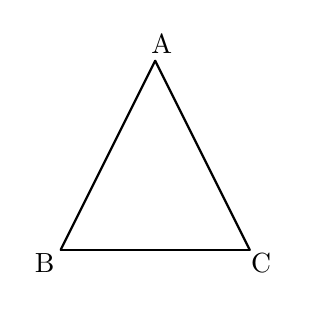
\begin{tikzpicture}[scale=0.6,line cap=round,line join=round,>=triangle 45,x=1.0cm,y=1.0cm]
\clip(-2.7,-0.7) rectangle (2.7,4.7);
\draw [line width=0.8pt] (0.,4.)-- (-2.,0.);
\draw [line width=0.8pt] (-2.,0.)-- (2.,0.);
\draw [line width=0.8pt] (2.,0.)-- (0.,4.);
\draw (0.14,4.37) node {A};
\draw (-2.34,-0.29) node {B};
\draw (2.24,-0.29) node {C};
\end{tikzpicture}
\end{center}
\end{multicols}

\vspace{8mm}

\begin{multicols}{2}

(\text{\refstepcounter{skaunta}%
\arabic{skaunta}})\hspace{2.5pt}(1)のあと、図を右のように変更した。このとき、$\triangle$ABCについて、二等辺三角形の底角が等しいことを証明することについて、正しいものを$\raise 0.2ex\hbox{\textcircled{\scriptsize{1}}}$または$\raise 0.2ex\hbox{\textcircled{\scriptsize{2}}}$から選びなさい。

\columnbreak

\begin{center}
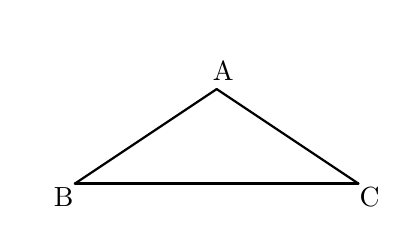
\begin{tikzpicture}[scale=0.6,line cap=round,line join=round,>=triangle 45,x=1.0cm,y=1.0cm]
\clip(-4,-0.7) rectangle (3.5,3.3);
\draw [line width=0.8pt] (0.,2)-- (-3,0.);
\draw [line width=0.8pt] (-3,0.)-- (3,0.);
\draw [line width=0.8pt] (3,0.)-- (0.,2);
\draw (0.14,2.4) node {A};
\draw (-3.24,-0.29) node {B};
\draw (3.24,-0.29) node {C};
\end{tikzpicture}
\end{center}

\end{multicols}

\begin{itemize}
\item[$\raise 0.2ex\hbox{\textcircled{\scriptsize{1}}}$]二等辺三角形の底角が等しいことをあらためて証明する必要がある。
\item[$\raise 0.2ex\hbox{\textcircled{\scriptsize{2}}}$]二等辺三角形の底角が等しいことは(1)で示されているので、あらためて証明する必要はない。
\end{itemize}


\vfill

\newpage

\setcounter{skaunta}{0}

\noindent\fbox{\large\makebox[1em]{\text{\refstepcounter{kaunta}%
\arabic{kaunta}}}} \hspace{1pt}次の太郎さんと花子さんの会話を読んで、各問に答えなさい。

%
\begin{flushright}%
\footnotesize{<(1)知・技4点、(2)思・判・表5点>}%
\end{flushright}%


\begin{screen}
\begin{itemize}
\item[太郎:] 世紀の大発見をしたよ!
\item[花子:] 世紀の大発見?
\item[太郎:] すべての三角形は二等辺三角形になるんだ。
\item[花子:] そんなはずはないよ。証明は?
\item[太郎:] もちろん証明したさ。
\item[花子:] 見せてみなさいよ。
\end{itemize}

\begin{itembox}[l]{証明}
\begin{multicols}{2}
右の$\triangle$ABCにおいて、$\angle$Aの二等分線とBCの垂直二等分線の交点をDとおく。DからAB, ACにおろした垂線の足をE, Fとおく。

このとき、直角三角形ADEとADFは斜辺と1つの鋭角がそれぞれ等しいので、$\triangle \mbox{ADE} \equiv \triangle \mbox{ADF}$。

よって、$\mbox{DE} = \mbox{DF}, \, \mbox{AE} = \mbox{AF}$。

\columnbreak

\begin{center}
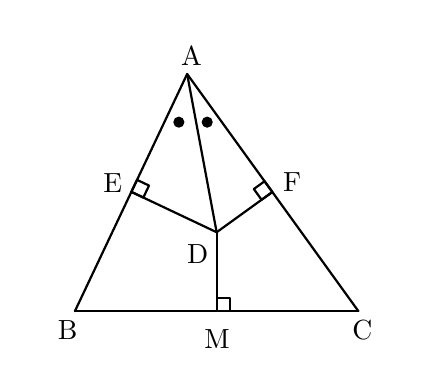
\begin{tikzpicture}[scale=1.2,line cap=round,line join=round,>=triangle 45,x=1.0cm,y=1.0cm]
\clip(-2.5,-0.5) rectangle (1.5,3.);
\draw[line width=0.8pt,fill opacity=0.10000000149011612] (-1.2757116906302963,1.2021063931759695) -- (-1.215646575974963,1.3290146823134439) -- (-1.3425548651124373,1.389079796968777) -- (-1.4026199797677705,1.2621715078313027) -- cycle; 
\draw[line width=0.8pt,fill opacity=0.10000000149011612] (0.007359912028126678,1.3745481058078255) -- (-0.10646691415103177,1.2923472208226945) -- (-0.024266029165900635,1.178520394643536) -- (0.08956079701325778,1.260721279628667) -- cycle; 
\draw[line width=0.8,fill opacity=0.10000000149011612] (-0.35959511457802085,0.) -- (-0.35959511457802085,0.14040488542197915) -- (-0.5,0.14040488542197915) -- (-0.5,0.) -- cycle; 
\draw [line width=0.8pt] (-0.8122606994077215,2.509509279129006)-- (-2.,0.);
\draw [line width=0.8pt] (-2.,0.)-- (1.,0.);
\draw [line width=0.8pt] (1.,0.)-- (-0.8122606994077215,2.509509279129006);
\draw [line width=0.8pt] (-0.8122606994077215,2.509509279129006)-- (-0.5,0.834965586583591);
\draw [line width=0.8pt] (-0.5,0.834965586583591)-- (-0.5,0.);
\draw [line width=0.8pt] (-0.5,0.834965586583591)-- (-1.4026199797677705,1.2621715078313027);
\draw [line width=0.8pt] (-0.5,0.834965586583591)-- (0.08956079701325778,1.260721279628667);
\draw[fill=black] (-0.6, 2.0) circle (1.5pt);
\draw[fill=black] (-0.9, 2.0) circle (1.5pt);
\draw (-0.7659294509973732,2.7) node {A};
\draw (-2.076441906032916,-0.2) node {B};
\draw (1.0409892370061777,-0.2) node {C};
\draw (-0.49456071030819515,-0.3) node {M};
\draw (-0.7,0.6) node {D};
\draw (-1.6,1.354537443756773) node {E};
\draw (0.3,1.3677749433025865) node {F};
\end{tikzpicture}

\end{center}

\end{multicols}

また、BCの中点をMとおくと、2組の辺とその間の角がそれぞれ等しいので、

$\triangle \mbox{DBM} \equiv \triangle \mbox{DCM}$。よって、$\mbox{DB} = \mbox{DC}$。

したがって、斜辺と他の一辺がそれぞれ等しいので、

$\triangle \mbox{DEB} \equiv \triangle \mbox{DFC}$。よって、$\mbox{EB} = \mbox{FC}$。

以上より、$\mbox{AB} = \mbox{AE} + \mbox{EB} = \mbox{AF} + \mbox{FC} = \mbox{AC}$

よって、$\triangle$ABCは$\mbox{AB} = \mbox{AC}$の二等辺三角形である。
\end{itembox}

\begin{itemize}
\item[花子:] たしかに...証明できているね。
\item[太郎:] そうでしょう?はい、おつかれ。解散解散。
\item[花子:] だけど、こんなパターンがあるでしょう。二等辺三角形じゃないよ...
\end{itemize}

\end{screen}

\begin{multicols}{2}

(\text{\refstepcounter{skaunta}%
\arabic{skaunta}})\hspace{2.5pt}花子さんは「すべての三角形が二等辺三角形である。」ことについて、右の$\triangle$ABCを使って反例をあげようとしています。解答欄の図に$\angle$Aの二等分線とBCの垂直二等分線を作図し、その交点をDとしなさい。。

\columnbreak

\begin{center}
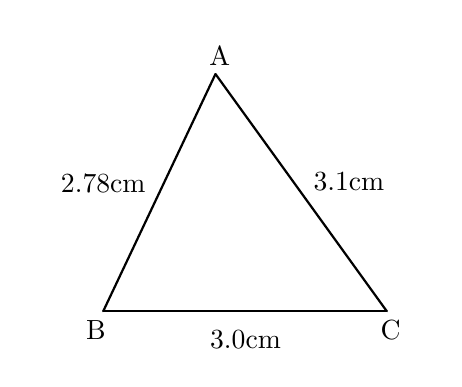
\begin{tikzpicture}[scale=1.2,line cap=round,line join=round,>=triangle 45,x=1.0cm,y=1.0cm]
\clip(-2.8,-0.5) rectangle (1.5,3.);
\draw [line width=0.8pt] (-0.8122606994077215,2.509509279129006)-- (-2.,0.);
\draw [line width=0.8pt] (-2.,0.)-- (1.,0.);
\draw [line width=0.8pt] (1.,0.)-- (-0.8122606994077215,2.509509279129006);
\draw (-0.7659294509973732,2.7) node {A};
\draw (-2.076441906032916,-0.2) node {B};
\draw (1.0409892370061777,-0.2) node {C};
\draw (-0.49456071030819515,-0.3) node {3.0cm};
\draw (-2.0,1.354537443756773) node {2.78cm};
\draw (0.6,1.3677749433025865) node {3.1cm};
\end{tikzpicture}
\end{center}

\end{multicols}

(\text{\refstepcounter{skaunta}%
\arabic{skaunta}})\hspace{2.5pt}(1)の結果から、太郎さんの証明において、間違っているのはどこか指摘しなさい。

\end{flushleft}

\end{document}
